
%% bare_jrnl.tex
%% V1.4b
%% 2015/08/26
%% by Michael Shell
%% see http://www.michaelshell.org/
%% for current contact information.
%%
%% This is a skeleton file demonstrating the use of IEEEtran.cls
%% (requires IEEEtran.cls version 1.8b or later) with an IEEE
%% journal paper.
%%
%% Support sites:
%% http://www.michaelshell.org/tex/ieeetran/
%% http://www.ctan.org/pkg/ieeetran
%% and
%% http://www.ieee.org/

%%*************************************************************************
%% Legal Notice:
%% This code is offered as-is without any warranty either expressed or
%% implied; without even the implied warranty of MERCHANTABILITY or
%% FITNESS FOR A PARTICULAR PURPOSE! 
%% User assumes all risk.
%% In no event shall the IEEE or any contributor to this code be liable for
%% any damages or losses, including, but not limited to, incidental,
%% consequential, or any other damages, resulting from the use or misuse
%% of any information contained here.
%%
%% All comments are the opinions of their respective authors and are not
%% necessarily endorsed by the IEEE.
%%
%% This work is distributed under the LaTeX Project Public License (LPPL)
%% ( http://www.latex-project.org/ ) version 1.3, and may be freely used,
%% distributed and modified. A copy of the LPPL, version 1.3, is included
%% in the base LaTeX documentation of all distributions of LaTeX released
%% 2003/12/01 or later.
%% Retain all contribution notices and credits.
%% ** Modified files should be clearly indicated as such, including  **
%% ** renaming them and changing author support contact information. **
%%*************************************************************************


% *** Authors should verify (and, if needed, correct) their LaTeX system  ***
% *** with the testflow diagnostic prior to trusting their LaTeX platform ***
% *** with production work. The IEEE's font choices and paper sizes can   ***
% *** trigger bugs that do not appear when using other class files.       ***                          ***
% The testflow support page is at:
% http://www.michaelshell.org/tex/testflow/



\documentclass[journal]{IEEEtran}
%
% If IEEEtran.cls has not been installed into the LaTeX system files,
% manually specify the path to it like:
% \documentclass[journal]{../sty/IEEEtran}


\usepackage{color}


% Some very useful LaTeX packages include:
% (uncomment the ones you want to load)


% *** MISC UTILITY PACKAGES ***
%
%\usepackage{ifpdf}
% Heiko Oberdiek's ifpdf.sty is very useful if you need conditional
% compilation based on whether the output is pdf or dvi.
% usage:
% \ifpdf
%   % pdf code
% \else
%   % dvi code
% \fi
% The latest version of ifpdf.sty can be obtained from:
% http://www.ctan.org/pkg/ifpdf
% Also, note that IEEEtran.cls V1.7 and later provides a builtin
% \ifCLASSINFOpdf conditional that works the same way.
% When switching from latex to pdflatex and vice-versa, the compiler may
% have to be run twice to clear warning/error messages.






% *** CITATION PACKAGES ***
%
%\usepackage{cite}
% cite.sty was written by Donald Arseneau
% V1.6 and later of IEEEtran pre-defines the format of the cite.sty package
% \cite{} output to follow that of the IEEE. Loading the cite package will
% result in citation numbers being automatically sorted and properly
% "compressed/ranged". e.g., [1], [9], [2], [7], [5], [6] without using
% cite.sty will become [1], [2], [5]--[7], [9] using cite.sty. cite.sty's
% \cite will automatically add leading space, if needed. Use cite.sty's
% noadjust option (cite.sty V3.8 and later) if you want to turn this off
% such as if a citation ever needs to be enclosed in parenthesis.
% cite.sty is already installed on most LaTeX systems. Be sure and use
% version 5.0 (2009-03-20) and later if using hyperref.sty.
% The latest version can be obtained at:
% http://www.ctan.org/pkg/cite
% The documentation is contained in the cite.sty file itself.






% *** GRAPHICS RELATED PACKAGES ***
%
\ifCLASSINFOpdf
  \usepackage[pdftex]{graphicx}
  % declare the path(s) where your graphic files are
  % \graphicspath{{../pdf/}{../jpeg/}}
  \graphicspath{{./}}
  % and their extensions so you won't have to specify these with
  % every instance of \includegraphics
  \DeclareGraphicsExtensions{.pdf,.jpeg,.png,PNG}
\else
  % or other class option (dvipsone, dvipdf, if not using dvips). graphicx
  % will default to the driver specified in the system graphics.cfg if no
  % driver is specified.
  % \usepackage[dvips]{graphicx}
  % declare the path(s) where your graphic files are
  % \graphicspath{{../eps/}}
  % and their extensions so you won't have to specify these with
  % every instance of \includegraphics
  % \DeclareGraphicsExtensions{.eps}
\fi
% graphicx was written by David Carlisle and Sebastian Rahtz. It is
% required if you want graphics, photos, etc. graphicx.sty is already
% installed on most LaTeX systems. The latest version and documentation
% can be obtained at: 
% http://www.ctan.org/pkg/graphicx
% Another good source of documentation is "Using Imported Graphics in
% LaTeX2e" by Keith Reckdahl which can be found at:
% http://www.ctan.org/pkg/epslatex
%
% latex, and pdflatex in dvi mode, support graphics in encapsulated
% postscript (.eps) format. pdflatex in pdf mode supports graphics
% in .pdf, .jpeg, .png and .mps (metapost) formats. Users should ensure
% that all non-photo figures use a vector format (.eps, .pdf, .mps) and
% not a bitmapped formats (.jpeg, .png). The IEEE frowns on bitmapped formats
% which can result in "jaggedy"/blurry rendering of lines and letters as
% well as large increases in file sizes.
%
% You can find documentation about the pdfTeX application at:
% http://www.tug.org/applications/pdftex





% *** MATH PACKAGES ***
%
%\usepackage{amsmath}
% A popular package from the American Mathematical Society that provides
% many useful and powerful commands for dealing with mathematics.
%
% Note that the amsmath package sets \interdisplaylinepenalty to 10000
% thus preventing page breaks from occurring within multiline equations. Use:
%\interdisplaylinepenalty=2500
% after loading amsmath to restore such page breaks as IEEEtran.cls normally
% does. amsmath.sty is already installed on most LaTeX systems. The latest
% version and documentation can be obtained at:
% http://www.ctan.org/pkg/amsmath





% *** SPECIALIZED LIST PACKAGES ***
%
\usepackage{algorithm}
\usepackage{algorithmic}
\usepackage{algpseudocode}
% algorithmic.sty was written by Peter Williams and Rogerio Brito.
% This package provides an algorithmic environment fo describing algorithms.
% You can use the algorithmic environment in-text or within a figure
% environment to provide for a floating algorithm. Do NOT use the algorithm
% floating environment provided by algorithm.sty (by the same authors) or
% algorithm2e.sty (by Christophe Fiorio) as the IEEE does not use dedicated
% algorithm float types and packages that provide these will not provide
% correct IEEE style captions. The latest version and documentation of
% algorithmic.sty can be obtained at:
% http://www.ctan.org/pkg/algorithms
% Also of interest may be the (relatively newer and more customizable)
% algorithmicx.sty package by Szasz Janos:
% http://www.ctan.org/pkg/algorithmicx




% *** ALIGNMENT PACKAGES ***
%
%\usepackage{array}
% Frank Mittelbach's and David Carlisle's array.sty patches and improves
% the standard LaTeX2e array and tabular environments to provide better
% appearance and additional user controls. As the default LaTeX2e table
% generation code is lacking to the point of almost being broken with
% respect to the quality of the end results, all users are strongly
% advised to use an enhanced (at the very least that provided by array.sty)
% set of table tools. array.sty is already installed on most systems. The
% latest version and documentation can be obtained at:
% http://www.ctan.org/pkg/array


% IEEEtran contains the IEEEeqnarray family of commands that can be used to
% generate multiline equations as well as matrices, tables, etc., of high
% quality.




% *** SUBFIGURE PACKAGES ***
%\ifCLASSOPTIONcompsoc
%  \usepackage[caption=false,font=normalsize,labelfont=sf,textfont=sf]{subfig}
%\else
%  \usepackage[caption=false,font=footnotesize]{subfig}
%\fi
% subfig.sty, written by Steven Douglas Cochran, is the modern replacement
% for subfigure.sty, the latter of which is no longer maintained and is
% incompatible with some LaTeX packages including fixltx2e. However,
% subfig.sty requires and automatically loads Axel Sommerfeldt's caption.sty
% which will override IEEEtran.cls' handling of captions and this will result
% in non-IEEE style figure/table captions. To prevent this problem, be sure
% and invoke subfig.sty's "caption=false" package option (available since
% subfig.sty version 1.3, 2005/06/28) as this is will preserve IEEEtran.cls
% handling of captions.
% Note that the Computer Society format requires a larger sans serif font
% than the serif footnote size font used in traditional IEEE formatting
% and thus the need to invoke different subfig.sty package options depending
% on whether compsoc mode has been enabled.
%
% The latest version and documentation of subfig.sty can be obtained at:
% http://www.ctan.org/pkg/subfig




% *** FLOAT PACKAGES ***
%
%\usepackage{fixltx2e}
% fixltx2e, the successor to the earlier fix2col.sty, was written by
% Frank Mittelbach and David Carlisle. This package corrects a few problems
% in the LaTeX2e kernel, the most notable of which is that in current
% LaTeX2e releases, the ordering of single and double column floats is not
% guaranteed to be preserved. Thus, an unpatched LaTeX2e can allow a
% single column figure to be placed prior to an earlier double column
% figure.
% Be aware that LaTeX2e kernels dated 2015 and later have fixltx2e.sty's
% corrections already built into the system in which case a warning will
% be issued if an attempt is made to load fixltx2e.sty as it is no longer
% needed.
% The latest version and documentation can be found at:
% http://www.ctan.org/pkg/fixltx2e


%\usepackage{stfloats}
% stfloats.sty was written by Sigitas Tolusis. This package gives LaTeX2e
% the ability to do double column floats at the bottom of the page as well
% as the top. (e.g., "\begin{figure*}[!b]" is not normally possible in
% LaTeX2e). It also provides a command:
%\fnbelowfloat
% to enable the placement of footnotes below bottom floats (the standard
% LaTeX2e kernel puts them above bottom floats). This is an invasive package
% which rewrites many portions of the LaTeX2e float routines. It may not work
% with other packages that modify the LaTeX2e float routines. The latest
% version and documentation can be obtained at:
% http://www.ctan.org/pkg/stfloats
% Do not use the stfloats baselinefloat ability as the IEEE does not allow
% \baselineskip to stretch. Authors submitting work to the IEEE should note
% that the IEEE rarely uses double column equations and that authors should try
% to avoid such use. Do not be tempted to use the cuted.sty or midfloat.sty
% packages (also by Sigitas Tolusis) as the IEEE does not format its papers in
% such ways.
% Do not attempt to use stfloats with fixltx2e as they are incompatible.
% Instead, use Morten Hogholm'a dblfloatfix which combines the features
% of both fixltx2e and stfloats:
%
% \usepackage{dblfloatfix}
% The latest version can be found at:
% http://www.ctan.org/pkg/dblfloatfix




%\ifCLASSOPTIONcaptionsoff
%  \usepackage[nomarkers]{endfloat}
% \let\MYoriglatexcaption\caption
% \renewcommand{\caption}[2][\relax]{\MYoriglatexcaption[#2]{#2}}
%\fi
% endfloat.sty was written by James Darrell McCauley, Jeff Goldberg and 
% Axel Sommerfeldt. This package may be useful when used in conjunction with 
% IEEEtran.cls'  captionsoff option. Some IEEE journals/societies require that
% submissions have lists of figures/tables at the end of the paper and that
% figures/tables without any captions are placed on a page by themselves at
% the end of the document. If needed, the draftcls IEEEtran class option or
% \CLASSINPUTbaselinestretch interface can be used to increase the line
% spacing as well. Be sure and use the nomarkers option of endfloat to
% prevent endfloat from "marking" where the figures would have been placed
% in the text. The two hack lines of code above are a slight modification of
% that suggested by in the endfloat docs (section 8.4.1) to ensure that
% the full captions always appear in the list of figures/tables - even if
% the user used the short optional argument of \caption[]{}.
% IEEE papers do not typically make use of \caption[]'s optional argument,
% so this should not be an issue. A similar trick can be used to disable
% captions of packages such as subfig.sty that lack options to turn off
% the subcaptions:
% For subfig.sty:
% \let\MYorigsubfloat\subfloat
% \renewcommand{\subfloat}[2][\relax]{\MYorigsubfloat[]{#2}}
% However, the above trick will not work if both optional arguments of
% the \subfloat command are used. Furthermore, there needs to be a
% description of each subfigure *somewhere* and endfloat does not add
% subfigure captions to its list of figures. Thus, the best approach is to
% avoid the use of subfigure captions (many IEEE journals avoid them anyway)
% and instead reference/explain all the subfigures within the main caption.
% The latest version of endfloat.sty and its documentation can obtained at:
% http://www.ctan.org/pkg/endfloat
%
% The IEEEtran \ifCLASSOPTIONcaptionsoff conditional can also be used
% later in the document, say, to conditionally put the References on a 
% page by themselves.




% *** PDF, URL AND HYPERLINK PACKAGES ***
%
%\usepackage{url}
% url.sty was written by Donald Arseneau. It provides better support for
% handling and breaking URLs. url.sty is already installed on most LaTeX
% systems. The latest version and documentation can be obtained at:
% http://www.ctan.org/pkg/url
% Basically, \url{my_url_here}.




% *** Do not adjust lengths that control margins, column widths, etc. ***
% *** Do not use packages that alter fonts (such as pslatex).         ***
% There should be no need to do such things with IEEEtran.cls V1.6 and later.
% (Unless specifically asked to do so by the journal or conference you plan
% to submit to, of course. )


% correct bad hyphenation here
\hyphenation{op-tical net-works semi-conduc-tor}


\begin{document}
%
% paper title
% Titles are generally capitalized except for words such as a, an, and, as,
% at, but, by, for, in, nor, of, on, or, the, to and up, which are usually
% not capitalized unless they are the first or last word of the title.
% Linebreaks \\ can be used within to get better formatting as desired.
% Do not put math or special symbols in the title.
\title{Sampling-Based Gaussian Estimation of Probability of Collision for Safe Planning}
%\title{The Theft of Labor by Automation}
%
%
% author names and IEEE memberships
% note positions of commas and nonbreaking spaces ( ~ ) LaTeX will not break
% a structure at a ~ so this keeps an author's name from being broken across
% two lines.
% use \thanks{} to gain access to the first footnote area
% a separate \thanks must be used for each paragraph as LaTeX2e's \thanks
% was not built to handle multiple paragraphs
%

\author{Ajaay~Chandrasekaran,~\IEEEmembership{\\Department of Electrical and Computer Engineering\\University of Michigan\\}Ann Arbor, Michigan 48109, U.S.A.\\Email: ajaay@umich.edu

%\author{Ajaay~Chandrasekaran,~\IEEEmembership{~Department of Electrical and Computer Engineering,}
%        John~Doe,~\IEEEmembership{Fellow,~OSA,}
%        and~Jane~Doe,~\IEEEmembership{Life~Fellow,~IEEE}% <-this % stops a space

%\thanks{M. Shell was with the Department
%of Electrical and Computer Engineering, Georgia Institute of Technology, Atlanta,
%GA, 30332 USA e-mail: (see http://www.michaelshell.org/contact.html).}% <-this % stops a space
%\thanks{J. Doe and J. Doe are with Anonymous University.}% <-this % stops a space
%\thanks{Manuscript received April 19, 2005; revised August 26, 2015.}

}

% note the % following the last \IEEEmembership and also \thanks - 
% these prevent an unwanted space from occurring between the last author name
% and the end of the author line. i.e., if you had this:
% 
% \author{....lastname \thanks{...} \thanks{...} }
%                     ^------------^------------^----Do not want these spaces!
%
% a space would be appended to the last name and could cause every name on that
% line to be shifted left slightly. This is one of those "LaTeX things". For
% instance, "\textbf{A} \textbf{B}" will typeset as "A B" not "AB". To get
% "AB" then you have to do: "\textbf{A}\textbf{B}"
% \thanks is no different in this regard, so shield the last } of each \thanks
% that ends a line with a % and do not let a space in before the next \thanks.
% Spaces after \IEEEmembership other than the last one are OK (and needed) as
% you are supposed to have spaces between the names. For what it is worth,
% this is a minor point as most people would not even notice if the said evil
% space somehow managed to creep in.



% The paper headers
%\markboth{Journal of \LaTeX\ Class Files,~Vol.~14, No.~8, August~2015}%
%{Shell \MakeLowercase{\textit{et al.}}: Bare Demo of IEEEtran.cls for IEEE Journals}
%\markboth{University of Michigan, ROB599: Robot Ethics, Final Paper, April~2018}%
%{Shell \MakeLowercase{\textit{et al.}}: Bare Demo of IEEEtran.cls for IEEE Journals}
% The only time the second header will appear is for the odd numbered pages
% after the title page when using the twoside option.
% 
% *** Note that you probably will NOT want to include the author's ***
% *** name in the headers of peer review papers.                   ***
% You can use \ifCLASSOPTIONpeerreview for conditional compilation here if
% you desire.




% If you want to put a publisher's ID mark on the page you can do it like
% this:
%\IEEEpubid{0000--0000/00\$00.00~\copyright~2015 IEEE}
% Remember, if you use this you must call \IEEEpubidadjcol in the second
% column for its text to clear the IEEEpubid mark.



% use for special paper notices
%\IEEEspecialpapernotice{(Invited Paper)}




% make the title area
\maketitle

% As a general rule, do not put math, special symbols or citations
% in the abstract or keywords.
\begin{abstract}
  This is the abstract.
\end{abstract}

% Note that keywords are not normally used for peerreview papers.
\begin{IEEEkeywords}
 collision probability, motion planning, safety, uncertainty.
\end{IEEEkeywords}

% For peer review papers, you can put extra information on the cover
% page as needed:
% \ifCLASSOPTIONpeerreview
% \begin{center} \bfseries EDICS Category: 3-BBND \end{center}
% \fi
%
% For peerreview papers, this IEEEtran command inserts a page break and
% creates the second title. It will be ignored for other modes.
\IEEEpeerreviewmaketitle


\section{Introduction}
% The very first letter is a 2 line initial drop letter followed
% by the rest of the first word in caps.
% 
% form to use if the first word consists of a single letter:
% \IEEEPARstart{A}{demo} file is ....
% 
% form to use if you need the single drop letter followed by
% normal text (unknown if ever used by the IEEE):
% \IEEEPARstart{A}{}demo file is ....
% 
% Some journals put the first two words in caps:
% \IEEEPARstart{T}{his demo} file is ....
% 
% Here we have the typical use of a "T" for an initial drop letter
% and "HIS" in caps to complete the first word.
\IEEEPARstart{T}he use of robots in elderly care is becoming increasingly likely throughout the world, as the population of elderly people is beginning to overtake the number of potential caregivers. 

\section{Related Work}

\section{Estimating Probability of Collision}
\subsection{Problem Statement}
We consider a robot operating in an environment with obstacles.% Our goal is to quantify the safety of a motion plan prior to its execution by the robot's controller. We quantify the safety of a plan via the probability that the robot will experience a collision while executing the plan.
The motion model of the robot is given as:
$$x_{t+1} = g(x_{t-1}, u_{t-1}, m), m \sim \mathcal{N}(0,R_t)$$
where $x_t \in \mathcal{C}$ is the configuration of the robot at time $t$, $u_t \in\mathbb{R}^{n_u}$ is the applied control input, and $m$ is a zero-mean Gaussian noise variable with variance $R_t$.

During execution of the motion plan, the robot obtains measurements of surrounding landmarks. The sensor model of the robot is given as:
$$z_t = h(x_t,l,n), n \sim \mathcal{N}(0,Q_t)$$
where $z_t \in \mathbb{R}^{n_z}$ is the measurement obtained at time $t$, $l \in \mathbb{R}^{n_l}$ is the location of the landmark that is observed, and $n$ is a zero-mean Gaussian noise variable with variance $Q_t$.

We assume the existence of a nominal plan computed by a motion planner. The nominal plan is defined by:
$$[x_0^*,u_0^*,...,x_N^*,u_N^*]$$
where $x_t^* = g(x_{t-1}^*,u_{t-1}^*,0)$ for $0 < t \leq N$ , where $N$ is the number of configurations in the motion plan.

With the preliminary notation established, we express our problem statement. Our goal is to estimate the probability of collision $p_c$ for the nominal plan. More formally, this probability is represented as:
$$p_c = p\left(\[ \bigvee\limits_{t=0}^N x_t^* \notin \mathcal{C}_F \]\right)$$
where $\mathcal{C}_F \subset \mathcal{C}$ represents the space of non-colliding configurations.

\subsection{Formulation and Assumptions}

Much of existing literature on this subect assumes that we can represent obstacles in the environment as known constraints on the robot's feasible locations in the workspace. However, we do not make that assumption, and we assume that there instead exists a collision checker $\phi: \mathcal{C} \rightarrow \{\text{TRUE},\text{FALSE}\}$, which can determine if a configuration is in collision. If $x\notin \mathcal{C}_F$, $\phi(x) = \text{TRUE}$; otherwise $\phi(x) = \text{FALSE}$ \cite{IEEEhowto:lavalle}.

The assumption of an available collision checker contrasts our formulation from other literatures, which tend to only consider point robots through the formulation of known robot location constraints based on obstacles. Our formulation lets us consider the possibility of non-point robots, whose locations in the workspace may cause collisions with obstacles due to the robots having 3D-geometries and being situated with complex orientations.

We assume that the Extended Kalman Filter (EKF) localization algorithm \cite{IEEEhowto:thrun} is used to compute $\hat{x_t}$, an estimate of the robot's true configuration, $x_t$, at time $t$. The covariance of the EKF estimate of $x_t$ is given by $\Sigma_t$. We assume that there is a set  of already known landmarks in the environment, $L = {l_1,...,l_{n_l}}$, where $n_l$ is the number of landmarks, and that data association between sensor measurements and landmarks is known.
%and that at each time $t$, the robot will receive measurements for all landmarks.

Due to the Gaussian noise in the motion model, we expect that the robot will deviate from the nominal motion plan during its execution. To compensate for the motion uncertainty, we assume that the robot operates with a closed-loop feedback controller \cite{IEEEhowto:stengel}. We assume that there exists a linear feedback control law that operates on the EKF estimate of the robot configuration and attempts to keep the robot close to the nominal plan. This feedback policy is given as:% related to the deviation of the estimate of the robot's configuration, $\hat{x_t}$, from the nominal configuration, $x_t^*$ as:
$$\bar{u_t} = L_{t+1}(\hat{x_t} - x_t^*) $$
where $L_{t}$ is the control gain matrix, which is contingent on the choice of feedback controller \cite{IEEEhowto:stengel} and $\bar{u_t}$ is the necessary deviation from the nominal control input $u_t^*$ to account for the robot's deviation from the nominal plan. It follows that $u_t = \bar{u_t} + u_t^*$, where $u_t$ represents the true control input to be executed by the robot--given the deviation of the robot's estimated configuration $\hat{x_t}$ from the nominal configuration $x_t^*$.

\subsection{Sources of Difficulty}
Computing the probability of collision for a motion plan in practice is a difficult task. There are three key sources of the difficulty:
\begin{enumerate}
\item Uncertainty in robot motion and sensor models
\item Dependent individual events of collision
\item Computational time of Monte-Carlo simulations
\end{enumerate}

We proceed to describe each of these sources.
\subsubsection{Model Uncertainty}
Robot motion is often corrupted by noise. We find that when we command a robot to follow a nominal control input, it often does not follow the command exactly due to various factors--usually wheel slippage due to lack of uniformity of surfaces.

Furthermore, sensor measurements that are used to localize a robot are also corrupted by natural noise and innaccuracy. Using sensor measurements for localization naturally causes uncertainty in the robot's known position. When using a state estimate as an input to a feedback control loop to correct the robot's position, there is a subsequent uncertainty in the accuracy of the desired controller adjustment--despite the desired intention of following the nominal motion plan.

\subsubsection{Dependence between Collision Events}
A key feature of this problem is that the event of a collision not occurring at a configuration $x_t$ of a motion plan is \underline{not} independent of the event of a collision not occurring at previous configurations of the motion plan. More formally:
$$p(x_t \in \mathcal{C}_F) \neq p\left(x_t \in \mathcal{C}_F | \bigwedge\limits_{i=0}^{t-1} x_i \in \mathcal{C}_F \right)$$

Prior approaches to solving this problem {\color{red}{cite here}} often consider the events of collisions along the motion plan to be independent of each other, which can lead to an overly conservative estimate of the probability of collision for a motion plan. Incorporating the fact that the collision events (and non-collision events) are dependent on each other increases the difficultly of computing an accurate estimate of the probability of collision.

\subsubsection{Computational Time of Monte-Carlo Simulations}

Running a large number of Monte-Carlo simulation, each having a large number of particles, can--in theory--give the true probability of collision for a motion plan. The idea of a Monte-Carlo simulation is to simulate the motion of thousands of particles, each particle representing a potential configuration of a robot's configuration given uncertainty in the robot's true configuration $x_t$. By finding the proportion of particles that did not collide with obstacles at all during the entirety of a motion plan, we can have an estimate of the probability of collision.

However, a single Monte-Carlo simulation is generally not sufficient, and we would need to average the proportions of colliding-particles across hundreds or even thousands of Monte-Carlo simulations to obtain an accurate estimate of the true probability of collision for the motion plan.

Furthermore, running a single Monte-Carlo simulation with thousands of particles can be very computationally expensive due to the compounding of time required for collision checking. Running thousands of Monte-Carlo simulations compounds the computation time even further, causing this approach to be a poor idea in practice.% In this case, computing the probability of collision for a motion plan would often require more time than that of computing the actual motion plan!

%This work attempts to enter the conversation regarding

\subsection{Metric Evaluation}
Given the sources of difficulty for this problem, we primarily strive to compute an \underline{accurate} estimate of the true probability of collision for a motion plan. We also seek to compute the probability of collision for the plan in an amount of time that is approximately less than or equal to the time required for a single Monte-Carlo simulation while within the error bounds of the average proportion of colliding particles that would be computed from executing hundreds of Monte-Carlo simulations with many particles in each simulation instance.

\begin{figure}[!t]
\centering
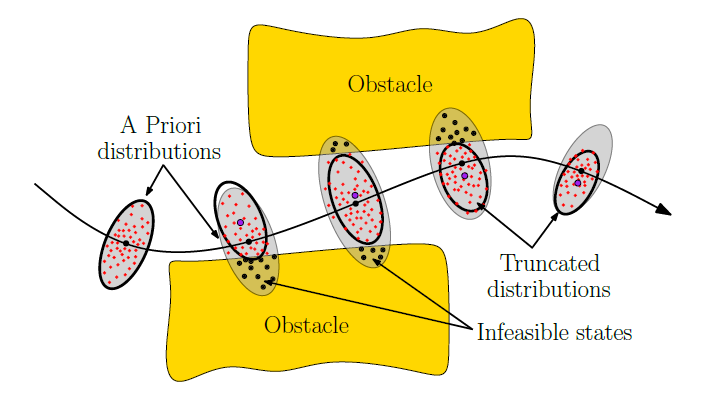
\includegraphics[width=3.5in]{motion_pic.PNG}
\caption{Propagation and Truncation of State Estimate Distribution. Figure borrowed from Patil, van den Berg, Alterovitz 2012. ``The probabilities of collision at each stage of the plan are conditioned on the previous stages being collision free. We truncate a priori distributions with respect to obstacles to discount plan executions that collide with obstacles (black disks). Propagating the truncated distributions (black ellipses) accounts for only the collision free samples (red disks), resulting in accurate estimation of the probability of collision. Using the unconditional distributions (gray ellipses) to estimate the collision probability results in a very conservative estimate.''\cite{IEEEhowto:patil}}
\label{patil_figure}
\end{figure}

\section{Method}
\subsection{Method Basis}

We propose a sampling-based method paired with the use of a Gaussian Mixture Model (GMM) to estimate the probability of collision for a motion plan. Our method adopts ideas from the the approach proposed by Patil, van den Berg, and Alterovitz \cite{IEEEhowto:patil}. However, our approach differs in that we do not assume that the environment obstacles can be represented as constraints on the robot location in the workspace, and we assume that a collision checker exists instead.

Figure \ref{patil_figure} portrays the approach recognized in \cite{IEEEhowto:patil}, which estimates the probability of collision for a motion plan by propagating a Kalman Filter (KF) estimate of a robot's state and truncating the distribution of the estimate with respect to obstacles. Patil et al. make the observation that the distribution of the robot's configuration at a timestep $t$--conditioned on the configuration $x_i \notin \mathcal{C}_F$, $\forall i, 0 \leq i < t $ being collision-free, can be represented by truncating the KF estimate at $x_t$ with respect to the obstacles. They also note that the proportion of the distribution that has been truncated by the obstacles would represent the conditional probability of collision for that state of the motion plan.

The approach of Patil et al. is purely analytical. It truncates the KF estimate of the robot state by sequentially applying each obstacle constraint to truncate the Gaussian distribution of the state estimate using analytical techniques from existing literature. They assume that the truncation of a Gaussian distribution by the obstacle constraints subsequently yields another Gaussian distribution.

The approach of Patil et al. makes two more important assumptions that are important to note when they truncate the KF estimate with respect to obstacles:
\begin{enumerate}
  \item The obstacles in the environment can be expressed as linear constraints on the robot's location in the workspace
  \item The free region containing the robot's configuration at time $t$ is convex
\end{enumerate}

We base our approach on the framework of \cite{IEEEhowto:patil}, and attempt to release these assumptions as we define our sampling-based GMM approach to estimate the probability of collision.

\subsection{Method Overview and Justification}

An important note to make is that the approach in \cite{IEEEhowto:patil} may be sufficient if we could express linear constraints in the configuration space $\mathcal{C}$ of a robot. Knowing the obstacle constraints in  $\mathcal{C}$ rather than as constraints on location in the robot's 3D-workspace could allow us to apply the approach of Patil et al. to truncate the distribution that represents a KF estimate of the robot's configuration. However, in general, computation of $\mathcal{C}_{OBS} \subset \mathcal{C}$, the space of all robot configurations that lead to collision with an obstacle, is computationally expensive in practice. It follows that learning configuration constraints in $\mathcal{C}$ rather than in the workspace may be very difficult in practice, as well. Furthermore, the constraints of $\mathcal{C}$ may also not be linear since $\mathcal{C}$ can have a complex topology.

Knowing (or learning) constraints for a robot's set of feasible configurations in $\mathcal{C}$ does not seem computationally efficient; however, we assume that we have access to the collision checker $\phi$, which asserts whether an arbitrary $x_t \in \mathcal{C}_{OBS}$. Given the existence of a collision checker, we believe that a \underline{sampling-based approach} for truncation of Gaussian distributions is necessary for a decent attempt of a solution to estimating the probability of collision. Other approaches assume the existence of a distance-to-obstacle checker {\color{red}{cite here}}, which may allow us to quantify the maximum clearance from an obstacle for a robot configuration to not collide. These approaches utilize this clearance in their computation of the probability of collision.

We observe that we need a method to truncate the robot state distribution computed from the KF estimate with respect to obstacles, where the proportion of the distribution that is truncated would represented the probability of collision for that waypoint of the motion plan--contingent on the the prior states being collision-free.

A straightforward approach using the collision checker involves sampling random configurations from the KF estimate of the robot's state and taking note of:
\begin{enumerate}
\item the proportion of sampled configurations in collision
\item the set of configurations that are not in collision
\end{enumerate}

%TODO: Something seems wrong here
Given 1, we would have an estimate, $p_{ct}$, for the probability of collision for that waypoint of the motion plan, and $1 - p_{ct}$ would represent the conditional probability of no collision, given that the previous states of the motion plan were collision-free. Given 2, we would be able to fit a distribution to the set of configurations that are not in collision, effectively truncating the original robot state distribution.

The left image of Figure \ref{ajaay_justification} portrays this approach where we attempt to fit a single Gaussian distribution to the set of robot configurations that are not in collision. We find that in extreme cases like this, a single Gaussian distribution may not best represent the distribution of non-colliding particles. This can be especially common if the feasible region in $\mathcal{C}$ containing $x_t$ is non-convex. Our approach recognizes this and proposes to truncate the distribution and represent the distribution of the subsequent set of non-colliding points as a mixture of Gaussians, or a GMM. We believe that the use of a GMM would more accurately capture the distribution of non-colliding configurations. The idea of this approach is demonstrated in the right image of Figure \ref{ajaay_justification}.

We also note that the approach in \cite{IEEEhowto:patil} degenerates when the free space containing the robot configuration is non-convex, as they use a greedy method to convexify the free space and obtain and overestimate of the probability of collision. This stems from their assumption that a single Gaussian distribution best represents the truncated distribution. We construct our GMM approach with the intention that it can handle these occurrences, representing the truncated distribution, as in the case of Figure \ref{ajaay_justification}, more accurately.


\begin{figure}[!t]
\centering
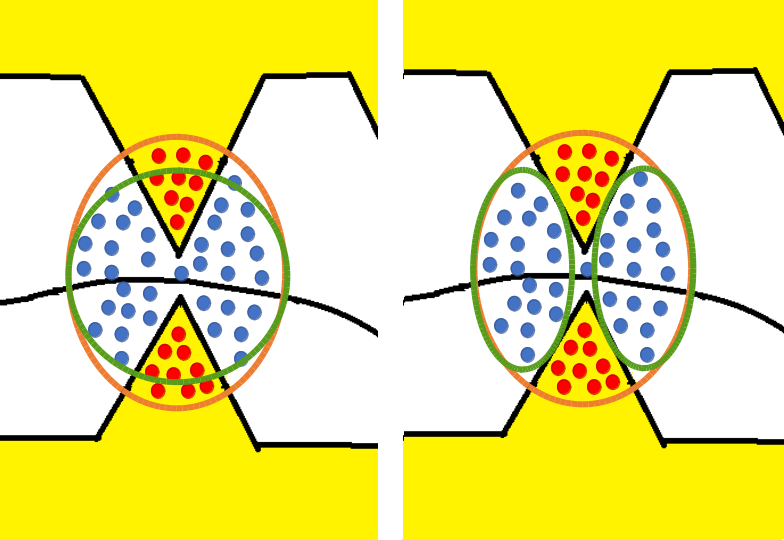
\includegraphics[width=3.5in]{combined_pic.png}
\caption{Our GMM approach attempts to handle situations where the distribution obtained by the truncation of the robot's configuration distribution by obstacles may not necessarily be represented sufficiently by a single Gaussian. [Left] When the EKF estimate of the robot's configuration (orange ellipse) is truncated, a single Gaussian distribution (green ellipse) may not best represent the subsequent collision-free distribution. [Right] A mixture of two Gaussians may represent the truncated collision-free distribution better than a single Gaussians.}
\label{ajaay_justification}
\end{figure}

\subsection{Algorithm}

Algorithm \ref{gmm_estim} portrays our sampling-based GMM collision probability estimation algorithm. The algorithm takes as input the nominal motion plan computed by a motion planner, $[x_0^*,u_0^*,...,x_N^*,u_N^*]$, and the initial configuration estimate $\mu_0$ and its covariance $\Sigma_0$. The algorithm also receives the number of Gaussians to use $N_G$, and the number of samples to take at each time step, $N_p$. 

\begin{figure*}[!t]
\centering
\subfloat (a) {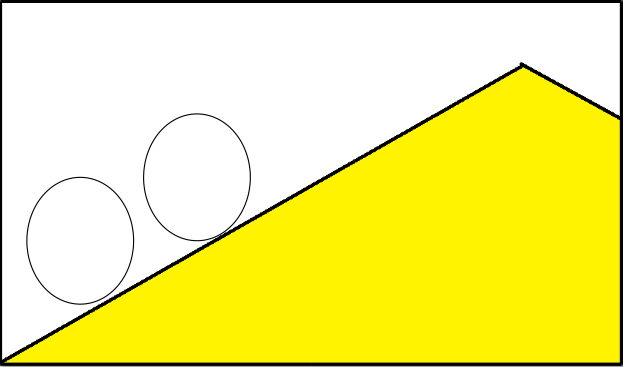
\includegraphics[width=1.55in]{step1.png}%
\label{step_one}}
\hfil
\subfloat (b) {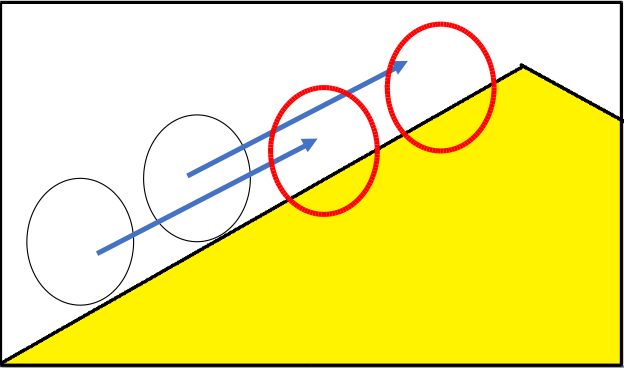
\includegraphics[width=1.55in]{step2.png}%
\label{step_two}}
\hfil
\subfloat (c) {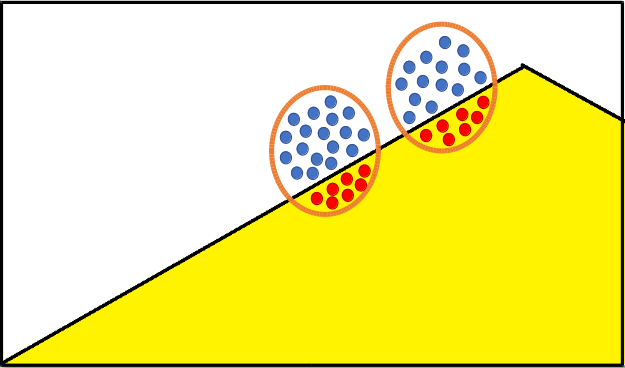
\includegraphics[width=1.55in]{step3.png}%
\label{step_three}}
\hfil
\subfloat (d) {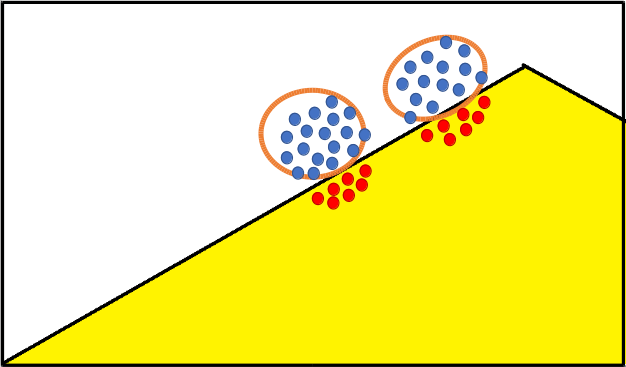
\includegraphics[width=1.55in]{step4.png}%
\label{step_four}}
\caption{Sampling-Based GMM Collision Estimation Algorithm applied to Mixture of 2 Gaussians. (a) Initialize mixture components with same initial mean $x_0^*$ and covariance $\Sigma_0$, as well as equal weights (Means shown as different here to highlight distinction). Gaussians are represented by blue ellipses. (b) Propagate Gaussians in mixture to next state of motion plan via EKF prediction step. Updated Gaussians are represented by red ellipses. (c) Update Gaussians via EKF correction step based on measurements (orange ellipses). Then, sample $N_p$ configurations from GMM based on weights. Check which configurations are in collision. Red dots represent colliding configurations and blue dots represent collision-free configurations. (d) Update mean and covariance of each Gaussian analytically based on the set of collision-free configurations contained in it. Update each mixture component's weight to be the proportion of the total non-colliding configurations that it contains.}
\label{algorithm_steps}
\end{figure*}

%\begin{figure*}[!t]
%\centering
%\subfloat[Case I]{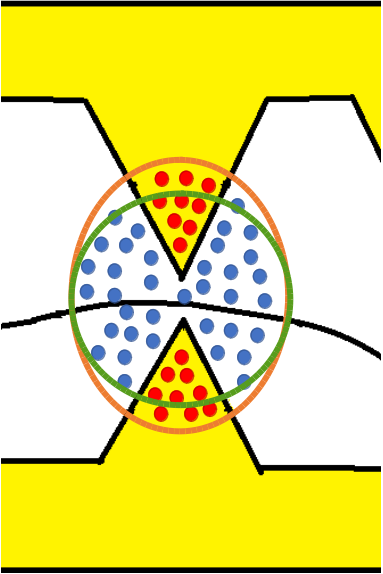
\includegraphics[width=0.5in]{one_gaussian.png}%
%\label{one_gauss}}
%\hfil
%\subfloat[Case II]{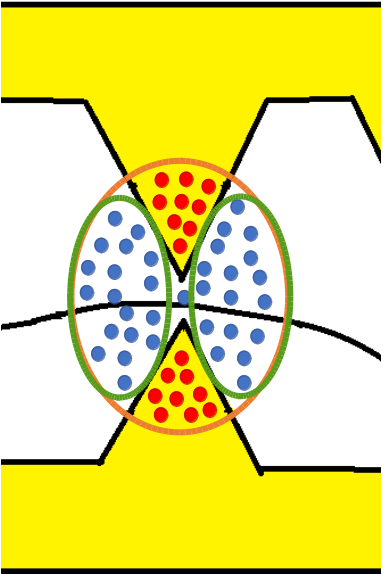
\includegraphics[width=0.5in]{two_gaussians.png}%
%\label{two_gauss}}
%\caption{Simulation results for the network.}
%\label{one_two_gauss}
%\end{figure*}

\renewcommand{\algorithmicrequire}{\textbf{Input:}}
\renewcommand{\algorithmicensure}{\textbf{Output:}}

\renewcommand{\algorithmicrequire}{\textbf{Input:}}
\renewcommand{\algorithmicensure}{\textbf{Output:}}

\begin{algorithm}
  \caption{Sampling-Based GMM Collision Estimation}
  \begin{algorithmic}[1]
    \REQUIRE{$[x_0^*,u_0^*,...,x_N^*,u_N^*], \mu_0,\Sigma_0, N_G, N_p$}
    \ENSURE{$p_c$}
    \STATE{$\mu^* \gets \mu_0$}
    \STATE{$\Sigma^* \gets \Sigma_0$}
    \STATE{$p_f \gets 1$}
    \STATE{$[\mu_1^*,\Sigma_1^*,...,\mu_{N_G}^*,\Sigma_{N_G}^*]$ $\gets$ INIT\_GMM($N_G, \mu_0,\Sigma_0$)}
    \STATE{$[\lambda_1,...,\lambda_{N_G}] \gets [\frac{1}{N_G},...,\frac{1}{N_G}]$}
    \FOR{$i = 0$ to $i = N-1$}
    \STATE{$\bar{u}_i \gets L_{t+1}(\mu^* - x_i^*)$}
    \STATE{$u_i \gets u_i^* + \bar{u}_i$}
    \STATE{$\bar{\mu}^*, \bar{\Sigma}^*$ $\gets$ EKF\_PREDICT($\mu^*,\Sigma^*,u_i$)}
    \STATE{$z_i$ $\gets$ SENSOR\_READ()}
    \STATE{${\mu}^*, {\Sigma}^*$ $\gets$ EKF\_CORRECT($\bar{\mu}^*,\bar{\Sigma}^*,z_i$)}
    
    \FOR{$j = 1$ to $j = N_G$}
    \STATE{$\bar{\mu}_i^*, \bar{\Sigma_i}^*$ $\gets$ EKF\_PREDICT($\mu_i^*,\Sigma_i^*,u_i$)}
    \STATE{${\mu}_i^*, {\Sigma}_i^*$ $\gets$ EKF\_CORRECT($\bar{\mu}_i^*,\bar{\Sigma}_i^*,z_i$)}
    
    \ENDFOR
    \STATE{$[\chi_1,...,\chi_{N_G}]$ $\gets$ SAMPLE\_GMM($N_p$)}
    \STATE{$C_c \gets 0$}
    \STATE{$[\bar{\chi_1},...\bar{\chi_{N_G}}] \gets [\emptyset,...,\emptyset]$}
    \FOR{$j = 1$ to $j = N_G$}
    \FOR{$q$ in $\chi_j$}
    \IF{CHECK\_COLLISION(q) == TRUE}
    $C_c \gets C_c + 1$
    \ELSE
    $\bar{\chi}_j \gets \{\bar{\chi}_j, q\}$
    \ENDIF
    %Check collision
    \ENDFOR
    %\STATE \texttt{<do stuff>}
    \ENDFOR

    \FOR{$j = 1$ to $j = N_G$}
    \STATE{$\mu_j^* \gets$ MEAN($\bar{\chi}_j$)}
    \STATE{$\Sigma_j^* \gets$ COVARIANCE($\bar{\chi}_j$)}
    \ENDFOR

    %Compute proportion of colliding articles
    \STATE{$p_i \gets \frac{C_c}{N_p}$}
    \STATE{$p_i \gets 1-p_i$}
    \STATE{$p_f \gets p_f * p_i$}
    \ENDFOR
    \STATE{$p_c \gets 1-p_f$}\\
  \end{algorithmic}
\label{gmm_estim}  
\end{algorithm}


\begin{algorithm}
  \caption{INIT\_GMM}
  \begin{algorithmic}[1]
    \REQUIRE{$[x_0^*,u_0^*,...,x_N^*,u_N^*]$}
    \ENSURE{$p_c$}
    \STATE{INIT\_GMM()}
    \IF{some condition is true}
      \STATE do some processing
    \ELSIF{some other condition is true}
      \STATE do some different processing
    \ELSIF{some even more bizarre condition is met}
      \STATE do something else
    \ELSE
      \STATE do the default actions
    \ENDIF
  \end{algorithmic}
\label{init_gmm}
\end{algorithm}

\section{Results}
Hi

\section{Discussion}

\section{Conclusion}

% An example of a floating figure using the graphicx package.
% Note that \label must occur AFTER (or within) \caption.
% For figures, \caption should occur after the \includegraphics.
% Note that IEEEtran v1.7 and later has special internal code that
% is designed to preserve the operation of \label within \caption
% even when the captionsoff option is in effect. However, because
% of issues like this, it may be the safest practice to put all your
% \label just after \caption rather than within \caption{}.
%
% Reminder: the "draftcls" or "draftclsnofoot", not "draft", class
% option should be used if it is desired that the figures are to be
% displayed while in draft mode.
%
%\begin{figure}[!t]
%\centering
%\includegraphics[width=2.5in]{myfigure}
% where an .eps filename suffix will be assumed under latex, 
% and a .pdf suffix will be assumed for pdflatex; or what has been declared
% via \DeclareGraphicsExtensions.
%\caption{Simulation results for the network.}
%\label{fig_sim}
%\end{figure}

% Note that the IEEE typically puts floats only at the top, even when this
% results in a large percentage of a column being occupied by floats.


% An example of a double column floating figure using two subfigures.
% (The subfig.sty package must be loaded for this to work.)
% The subfigure \label commands are set within each subfloat command,
% and the \label for the overall figure must come after \caption.
% \hfil is used as a separator to get equal spacing.
% Watch out that the combined width of all the subfigures on a 
% line do not exceed the text width or a line break will occur.
%
%\begin{figure*}[!t]
%\centering
%\subfloat[Case I]{\includegraphics[width=2.5in]{box}%
%\label{fig_first_case}}
%\hfil
%\subfloat[Case II]{\includegraphics[width=2.5in]{box}%
%\label{fig_second_case}}
%\caption{Simulation results for the network.}
%\label{fig_sim}
%\end{figure*}
%
% Note that often IEEE papers with subfigures do not employ subfigure
% captions (using the optional argument to \subfloat[]), but instead will
% reference/describe all of them (a), (b), etc., within the main caption.
% Be aware that for subfig.sty to generate the (a), (b), etc., subfigure
% labels, the optional argument to \subfloat must be present. If a
% subcaption is not desired, just leave its contents blank,
% e.g., \subfloat[].


% An example of a floating table. Note that, for IEEE style tables, the
% \caption command should come BEFORE the table and, given that table
% captions serve much like titles, are usually capitalized except for words
% such as a, an, and, as, at, but, by, for, in, nor, of, on, or, the, to
% and up, which are usually not capitalized unless they are the first or
% last word of the caption. Table text will default to \footnotesize as
% the IEEE normally uses this smaller font for tables.
% The \label must come after \caption as always.
%
%\begin{table}[!t]
%% increase table row spacing, adjust to taste
%\renewcommand{\arraystretch}{1.3}
% if using array.sty, it might be a good idea to tweak the value of
% \extrarowheight as needed to properly center the text within the cells
%\caption{An Example of a Table}
%\label{table_example}
%\centering
%% Some packages, such as MDW tools, offer better commands for making tables
%% than the plain LaTeX2e tabular which is used here.
%\begin{tabular}{|c||c|}
%\hline
%One & Two\\
%\hline
%Three & Four\\
%\hline
%\end{tabular}
%\end{table}


% Note that the IEEE does not put floats in the very first column
% - or typically anywhere on the first page for that matter. Also,
% in-text middle ("here") positioning is typically not used, but it
% is allowed and encouraged for Computer Society conferences (but
% not Computer Society journals). Most IEEE journals/conferences use
% top floats exclusively. 
% Note that, LaTeX2e, unlike IEEE journals/conferences, places
% footnotes above bottom floats. This can be corrected via the
% \fnbelowfloat command of the stfloats package.


% if have a single appendix:
%\appendix[Proof of the Zonklar Equations]
% or
%\appendix  % for no appendix heading
% do not use \section anymore after \appendix, only \section*
% is possibly needed

% use appendices with more than one appendix
% then use \section to start each appendix
% you must declare a \section before using any
% \subsection or using \label (\appendices by itself
% starts a section numbered zero.)
%


%I commented this, don't need appendices (AJAAY)

%\appendices
%\section{Proof of the First Zonklar Equation}
%Appendix one text goes here.

% you can choose not to have a title for an appendix
% if you want by leaving the argument blank
%\section{}
%Appendix two text goes here.


% use section* for acknowledgment
\section*{Acknowledgment}
The author would like to acknowledge Dmitry Berenson, Maani Ghaffari, and Valerie Chen for their helpful feedback.

% Can use something like this to put references on a page
% by themselves when using endfloat and the captionsoff option.
\ifCLASSOPTIONcaptionsoff
  \newpage
\fi



% trigger a \newpage just before the given reference
% number - used to balance the columns on the last page
% adjust value as needed - may need to be readjusted if
% the document is modified later
%\IEEEtriggeratref{8}
% The "triggered" command can be changed if desired:
%\IEEEtriggercmd{\enlargethispage{-5in}}

% references section

% can use a bibliography generated by BibTeX as a .bbl file
% BibTeX documentation can be easily obtained at:
% http://mirror.ctan.org/biblio/bibtex/contrib/doc/
% The IEEEtran BibTeX style support page is at:
% http://www.michaelshell.org/tex/ieeetran/bibtex/
%\bibliographystyle{IEEEtran}
% argument is your BibTeX string definitions and bibliography database(s)
%\bibliography{IEEEabrv,../bib/paper}
%
% <OR> manually copy in the resultant .bbl file
% set second argument of \begin to the number of references
% (used to reserve space for the reference number labels box)
\begin{thebibliography}{1}

%\bibitem{IEEEhowto:kopka}H.~Kopka and P.~W. Daly, \emph{A Guide to \LaTeX}, 3rd~ed.\hskip 1em plus
%  0.5em minus 0.4em\relax Harlow, England: Addison-Wesley, 1999.

\bibitem{IEEEhowto:lavalle} S.~LaValle. \emph{Planning Algorithms}. Cambridge University Press, 2006.
\bibitem{IEEEhowto:patil} S. Patil, J. van den Berg, and R. Alterovitz, “Estimating probability of collision for safe planning under Gaussian motion and sensing uncertainty,” in ICRA, 2012, pp. 3238-3244.
\bibitem{IEEEhowto:stengel} R.~F.~Stengel, \emph{Optimal Control and Estimation}. Dover Publications, 1994.
\bibitem{IEEEhowto:thrun} S.~Thrun, W.~Burgard, and D.~Fox. \emph{Probabilistic Robotics}. MIT Press, 2005.

\end{thebibliography}

% biography section
% 
% If you have an EPS/PDF photo (graphicx package needed) extra braces are
% needed around the contents of the optional argument to biography to prevent
% the LaTeX parser from getting confused when it sees the complicated
% \includegraphics command within an optional argument. (You could create
% your own custom macro containing the \includegraphics command to make things
% simpler here.)
%\begin{IEEEbiography}[{\includegraphics[width=1in,height=1.25in,clip,keepaspectratio]{mshell}}]{Michael Shell}
% or if you just want to reserve a space for a photo:


%Picture biography, uncomment this if you want a photo
%\begin{IEEEbiography}{Ajaay Chandrasekaran}
\begin{IEEEbiographynophoto}{Ajaay Chandrasekaran}
  received the BSE degree in computer science from the University of Michigan, Ann Arbor, MI, in 2017.
  He is currently pursuing the MSE degree in electrical and computer engineering from the University of Michigan.% His primary research interests include robotic motion planning under uncertainty and perception and planning for autonomous vehicles.
\end{IEEEbiographynophoto}

\vfill

% if you will not have a photo at all:
%\begin{IEEEbiographynophoto}{John Doe}
%Biography text here.
%\end{IEEEbiographynophoto}

% insert where needed to balance the two columns on the last page with
% biographies
%\newpage

%\begin{IEEEbiographynophoto}{Jane Doe}
%Biography text here.
%\end{IEEEbiographynophoto}

% You can push biographies down or up by placing
% a \vfill before or after them. The appropriate
% use of \vfill depends on what kind of text is
% on the last page and whether or not the columns
% are being equalized.

%\vfill

% Can be used to pull up biographies so that the bottom of the last one
% is flush with the other column.
%\enlargethispage{-5in}



% that's all folks
\end{document}


